\section{Results}
    \subsection{Usability Results}
        \paragraph{}
        After several attempts of trying different UI designs for the best user experience in regards to the usability of the calculator, we’ve concluded that the best experience would be a dark scientific look that includes the calculation history. As many software calculators may have this classic look and layout, we have a few key features that enhance the use of this calculator compared to most similar software calculators in today's market.

        \begin{center}
            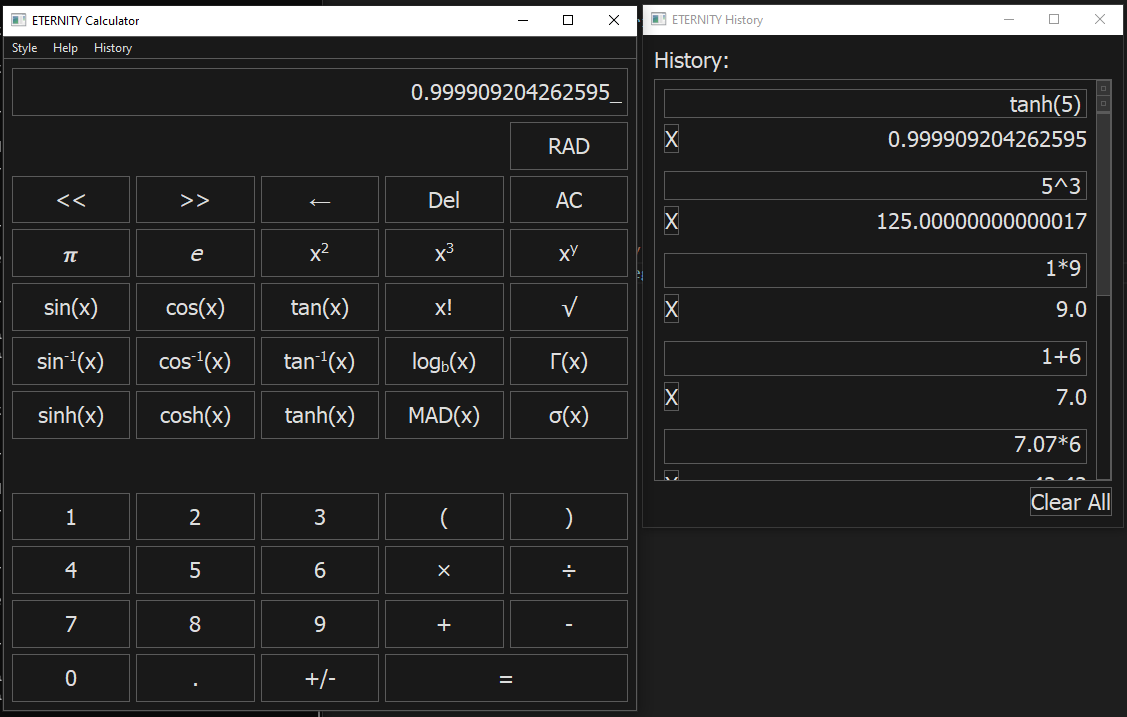
\includegraphics[scale=0.3]{images/usability}
        \end{center}

        \paragraph{}
        Similar to the explanation in the UI design section, we wanted to make sure that the user will always know the difference between the scientific functions and the normal input functions such as the addition, subtraction, etc. We’ve even added a blank separator that will reduce the confusion while keeping the scientific functions to the top and the basic functions to the bottom. In an unanimous agreement, the equal button should be the largest button for the user where they should be able to detect easily after inputting the calculations they need.

        \paragraph{}
        The accuracy of the results with our scientific functions is one of our most fundamental goals in the creation of the calculator. Throughout our team, we each had the responsibility in producing our own functions that were assigned by our team members. Everyone has done an excellent job where for example, the marginal error from an Arccos(x) function would be 0.00000000001 in radians of a difference in comparison to the imported math function. This will give the confidence to any user whether they are in construction or in sales that the numbers will be accurate even if their computer literacy is very low.

    \subsection{Test Results}
        \paragraph{}
        Each functionalities were tested in their own way to make sure that the result of the calculator was as accurate as possible. To achieve this, tests were created for each function, and the results of each test were compared to results that were found using a trusted source, which was, in this case, the equivalent python functions. Because we know that the Python source code needs to be accurate as much as possible, we know that they answer are reliable enough to make sure that our tests are also reliable.

        \paragraph{}
        For example, to test if the exponent function works correctly, we first pick a lot of numbers to test, which makes sure that we cover as many edge cases as possible. Then, we calculate the exponents using those numbers using both the built-in Python functions, and our own functions, and we compare the results. Doing this for all functions allows us to be sure of our results.

    \subsection{Evaluation Results}
        \paragraph{}
        With three months of work, we were able to create our fully functional software calculator. As mentioned in the usability results, the accuracy of the functions that our team programmed is extremely accurate in regards to the built in math functions. Any user can download this calculator and use it right after launching the program. There are a couple of things we did want to include, however the team just didn’t have enough time to implement them while meeting the deadline. We wanted to have a dedicated unit conversions button, similar to the RAD and degree button. This feature would have helped more users that need to quickly convert the results to a different unit such as inches to centimeters. We also wanted to make it mobile friendly, however, we did not have the chance to import it to a phone. We did however meet the main objective which is to build a software calculator that can be used in dark mode and help our interviewees by creating a calculator that solves problems related to their industry. We are proud of what we were able to achieve as some of our teammates have been studying while also working full time.


    \subsection{Test Cases}
        \begin{enumerate}
            \item Task: Use History to repeat an inputted math expression
            \begin{enumerate}
                \item Calculate 1+2. The result should be equal to 3.
                \item Calculate 3*4. The result should be 12.
                \item Open the History window by clicking on History on the menu. In the pop up window, there will be the 2 equations, and their results.
                \item Click on any empty space of the 1+2 equation. The equation will be written back on the calculator in the expression box, where it can be calculated again or modified.
            \end{enumerate}

            \item Task: Evaluate standard deviation of grades of COMP 354 Deliverable 2
            \begin{enumerate}
                    \item Press on the standard deviation button ($\sigma$).
                    \item A pop up window appears asking for a comma separated set of numbers
                    \item Enter data points of grades acquired by individual students of a class as a comma separated list in the pop up window. Deliverable 2 had following marks: 36.67, 36.67, 36, 37.33, 39.67, 36.67, 35, 38.67, 38.67, 35.33, 39, 38.33
                    \item Press the ok button at the bottom of the pop up window
                    \item The list is inputted into the expression box. Press the Equals button to calculate the Standard Deviation of the data points.
                    \item Standard deviation for deliverable 2 marks is 1.4537334598275653
                \end{enumerate}

            \item Task: Evaluate $log2(3) * log4(8)$
                \begin{enumerate}
                	\item Press on log button
                	\item Press the << to move the cursor 1 to the left
                	\item Enter your base (2)
                	\item Press the >> to move the cursor 1 to the right
                	\item Enter your value (3)
                	\item Press the >> to move the cursor 1 to the right
                	\item Press the * button
                	\item Press on log button
                	\item Press the << to move the cursor 1 to the left
                	\item Enter your base (4)
                	\item Press the >> to move the cursor 1 to the right
                	\item Enter your value (3)
                	\item Press the >> to move the cursor 1 to the right
                    \item Press the = button to complete the calculation. The result should be 2.37744375
                \end{enumerate}

            \item Task: Evaluate $sinh(2)*5$.
                \begin{enumerate}
                    \item Press on the $sinh$ button
                    \item Enter the value 2. Expression is sinh(2)
                	\item Press the >> to move the cursor 1 to the right
                    \item Press the * button (multiplication)
                    \item Enter the value 5. Expression is $sinh(2)*5$
                    \item Press the equals button. This evaluates  $sinh(2)*5$. Result should be approximately 18.1343.
                \end{enumerate}

            \item Task: Evaluate Arccos(.5)
                \begin{enumerate}
                    \item Make sure that the calculator is reset to zero by pressing AC.
                	\item Click on the Arccos(x) button which looks like this: $cos^(-1)(x)$
                    \item Click and enter the point (.) button located between the zero (0) and the plus/minus (+/-) button.
                    \item Now click and enter the value 5 button located in between the four (4) and six (6) horizontally.
                    \item Click on the equal (=) button.
                    Step 6. The value should be 1.047197551 in radians.
                \end{enumerate}


            \item Task: Evaluate MAD([1, 2, 3, 4, 5])
                \begin{enumerate}
                    \item Click on the Mean Average Deviation (MAD) button.
                    \item A window will pop up asking for a list of values
                    \item Enter the values: 1, 2, 3, 4, 5 as a comma separated list of numbers.
                    \item Press on the Ok button at the bottom of the popped up window. The list is inputted into the expression box.
                    \item Click on the Equals button (=) to get the final answer as 1.2
                \end{enumerate}

            \item Task: Evaluate $\gamma(3)+10$.
                \begin{enumerate}
                	\item Click on the Gamma Function $\gamma(x)$ button.
                	\item Enter the value 3 by clicking on the button 3.
                	\item Click the >> button to move the cursor to the right most position.
                	\item Click the + (addition) button.
                	\item Enter the value 10 by clicking on the button 1 then 0.
                	\item Click the Equals button (=) to get the final answer as 12.0.
                \end{enumerate}
        \end{enumerate}
